% !TEX root = ../../thesis.tex

\documentclass[../../thesis.tex]{subfiles}
 
\begin{document}

In this chapter, we experiment with our solvers and discuss the results. 

\section{Benchmark process}

We used our benchmark runner described in \autoref{section:benchmark-runner} to run our experiments.
Once all the tested solvers have finished their run, we extract the results and create a JSON file 
with the final results (objective, time, etc.). We can then create plots that make it 
easier to analyze and discuss the results. Two of those plots are \emph{timelines} and \emph{performance profiles}.

\subsection{Timelines}

A timeline is a decreasing function of the objective over time. 
They represent the average evolution of the objective of all instances over time.
However, as objectives can be 
significantly different from one instance to another, all objectives are normalized to a $[0, 1]$ range.
We call this the relative distance to the best objective. 
The normalized objective ($no$) for instance $i$ at each timestamp $t$ can 
be computed with the following formula:

\begin{equation*}
  no_i(t) = \frac{objective_i(t) - best_i}{objective_i(0) - best_i}
\end{equation*}

A value of $1$ will always be the initial solution for each solver, even though they might not be equal. A value of 
$0$ is the best solution found at the end of the search. 

For each time $t$, we take the average of all normalized objectives over all instances:


\begin{equation*}
   no(t) = \frac{\sum_{i \in \mathcal{I}} no_{i}(t)}{|\mathcal{I}|}
\end{equation*}



\begin{figure}
  \centering
  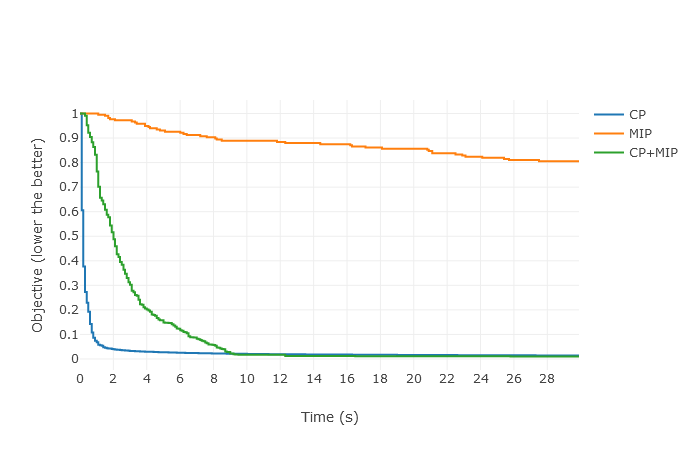
\includegraphics[scale=0.50]{experiments/solvers-oot.png}
  \caption{Example of a timeline.}
  \label{timeline-example}
\end{figure}

\autoref{timeline-example} shows an example of a timeline with three solvers. The $x$ axis is the time in seconds and the $y$ axis is the normalized objective 
value. In practice, we do not compute the normalized objective for every second but for every 1/10th second for more accurate results.



\subsection{Performance profiles}

A performance profile \cite{Dolan2002} is a cumulative distribution function of a performance metric (i.e. objective, time, etc.).
In our case, we are mostly interested in the objective metric after a fixed amount of time.
This is how a performance profile is computed:

For each problem $p$ and solver $s$, we define two performance metrics:

\begin{align*}
  t_{p, s} &= \text{time required to solve $p$ by solver $s$} \\
  o_{p, s} &= \text{objective of $p$ obtained by solver $s$}
\end{align*}


From these results, we can compute a performance ratio $r_{p, s}$ for a performance metric.
We use $m_{p, s}$ in the following formulas which refers to a performance metric such as $t_{p, s}$ or $o_{p, s}$.

\begin{equation}
  r_{p, s} = \frac{m_{p, s}}{min\{ m_{p, s} : s \in \mathcal{S} \}}
\end{equation}

This ratio is the comparison between the performance of a solver $s$ with the best solver for $p$.
This means that the best solver is used as baseline. However, it can be interesting to change 
the baseline to change the comparison. For this, we change the formula \cite{Cauwelaert2017AVW} to:

\begin{equation}
  r_{p, s} = \frac{m_{p, s}}{min\{ m_{p, b} : b \in \mathcal{B} \} }
\end{equation}

where $\mathcal{B} \subseteq \mathcal{S}$ is the set of baselines.
The performance profile of a solver is then given by:


\begin{equation}
  F_s(\tau) = \frac{1}{|\mathcal{P}|} \left| \left\{ p \in \mathcal{P} : r_{p, s} \leq \tau \right\} \right|
\end{equation}

with $\tau \in \mathbb{R}$ being a performance factor. In other words, $F_s(\tau)$ is the cumulative probability
of having a performance ratio within a factor $\tau$ of the best possible ratio.

\begin{figure}
  \centering
  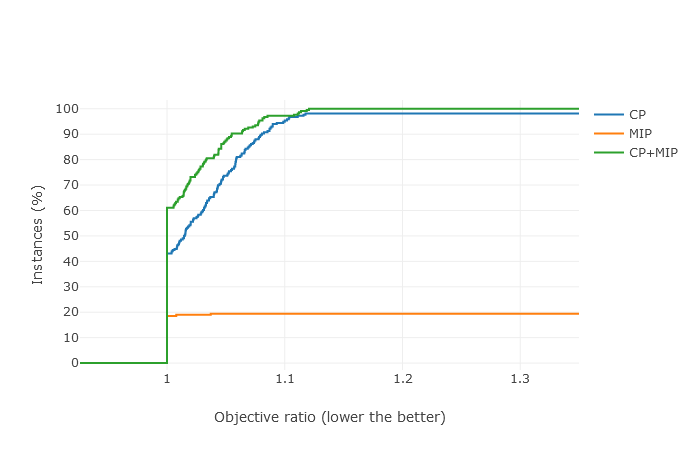
\includegraphics[scale=0.55]{experiments/solvers-profile-zoom.png}
  \caption{Example of performance profiles.}
  \label{example-profile}
\end{figure}

We can plot multiple performance profiles of different solvers, with different baselines, to compare them.
\autoref{example-profile} shows an example of performance profiles with the objective as performance metric.
These profiles represent the objective after a fixed amount of time 
with two solvers CP and CP+MIP with CP as 
baseline.
We can see on the $y$ axis the percentage of instances solved by the solvers and on the $x$ the objective expressed
as a ratio of the objective obtained by the baseline. We can see in this example that for around 60\% of instances,
the objective is better or equal for the CP+MIP solver with an improvement of up to 10\% compared to the baseline.
In the remaining 40\% of instances, we can see that the CP+MIP solver is worse also up to around 10\%.


We can also have multiple solvers as baseline as we can see in \autoref{example-profile2} where all the solvers 
are used as baselines. In this type of profile, the objective used in the objective ratio is the best objective between all solvers.

\begin{figure}
  \centering
  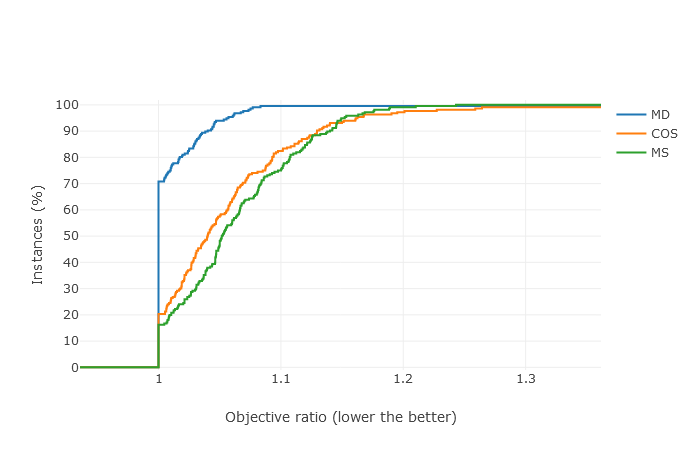
\includegraphics[scale=0.55]{experiments/v-heuristics-profile.png}
  \caption{Example of performance profiles with all solvers as baselines.}
  \label{example-profile2}
\end{figure}


\subsection{Hardware}

All the experiments were performed on a UCLouvain server \cite{jabba} from the INGI department.

\begin{itemize}
  \item Intel(R) Xeon(R) CPU E5-2687W v3 \verb+@+ 3.10GHz 
    \begin{itemize}
      \item 20 cores available.
      \item 40 threads.
    \end{itemize}
  \item 128 Go RAM
\end{itemize}

The tests were run mostly during the night due to the long running times and to avoid having 
perturbations from other users. However, as this machine has a high number of cores, running tests 
during the day did not impact the results. 
The server load was monitored through the INGI website \cite{jabba:monitoring} and the server was never noticed to be overloaded.

\subsection{Benchmark instances}

For our experiments, we generated 216 instances of different sizes. The problem sizes were based on the needs of the \vone\ company.
\autoref{instances:proportions} shows the size proportions for the 216 instances used in the experiments. $T$ represents the number of time period, $D$ the number of demands and $W$ the number of workers. The generated instances also have varying probabilities as presented in \autoref{instance:options}. These probabilities are referenced in \autoref{instances:probabilities} and follow a uniform distribution where $P_{\mu} = \frac{P_{min} + P_{max}}{2}$.


\begin{table}[H]
  \caption{Proportions of instance sizes for 216 instances.}
  \label{instances:proportions}
  \centering
  \begin{tabular}[t]{|c|c|c |c|c|}
    \hline
    \multicolumn{3}{|c|}{Size} & \multicolumn{2}{|c|}{Prop.} \\
    \hline 
    $T$ & $D$ & $W$ & $n$ & $\%$ \\
    \hline 
    \multirow{9}{*}{5} & \multirow{3}{*}{30} & 150 & 8 & 3.7 \\ 
    \cline{3-5}
     &  & 225 & 8 & 3.7 \\ 
     \cline{3-5}
     &  & 300 & 8 & 3.7 \\ 
     \cline{2-5}
     & \multirow{3}{*}{40} & 150 & 8 & 3.7 \\ 
     \cline{3-5}
     &  & 225 & 8 & 3.7 \\ 
     \cline{3-5}
     &  & 300 & 8 & 3.7 \\ 
     \cline{2-5}
     & \multirow{3}{*}{50} & 150 & 8 & 3.7 \\ 
     \cline{3-5}
     &  & 225 & 8 & 3.7 \\ 
     \cline{3-5}
     &  & 300 & 8 & 3.7 \\ 
    \hline
  \end{tabular}
  \hfill
  \begin{tabular}[t]{|c|c|c |c|c|}
    \hline
    \multicolumn{3}{|c|}{Size} & \multicolumn{2}{|c|}{Prop.} \\
    \hline 
    $T$ & $D$ & $W$ & $n$ & $\%$ \\
    \hline 
    \multirow{9}{*}{10} & \multirow{3}{*}{30} & 150 & 8 & 3.7 \\ 
    \cline{3-5}
     &  & 225 & 8 & 3.7 \\ 
     \cline{3-5}
     &  & 300 & 8 & 3.7 \\ 
     \cline{2-5}
     & \multirow{3}{*}{40} & 150 & 8 & 3.7 \\ 
     \cline{3-5}
     &  & 225 & 8 & 3.7 \\ 
     \cline{3-5}
     &  & 300 & 8 & 3.7 \\ 
     \cline{2-5}
     & \multirow{3}{*}{50} & 150 & 8 & 3.7 \\ 
     \cline{3-5}
     &  & 225 & 8 & 3.7 \\ 
     \cline{3-5}
     &  & 300 & 8 & 3.7 \\ 
    \hline
  \end{tabular}
  \hfill
  \begin{tabular}[t]{|c|c|c |c|c|}
    \hline
    \multicolumn{3}{|c|}{Size} & \multicolumn{2}{|c|}{Prop.} \\
    \hline 
    $T$ & $D$ & $W$ & $n$ & $\%$ \\
    \hline 
    \multirow{9}{*}{15} & \multirow{3}{*}{30} & 150 & 8 & 3.7 \\ 
    \cline{3-5}
     &  & 225 & 8 & 3.7 \\ 
     \cline{3-5}
     &  & 300 & 8 & 3.7 \\ 
     \cline{2-5}
     & \multirow{3}{*}{40} & 150 & 8 & 3.7 \\ 
     \cline{3-5}
     &  & 225 & 8 & 3.7 \\ 
     \cline{3-5}
     &  & 300 & 8 & 3.7 \\ 
     \cline{2-5}
     & \multirow{3}{*}{50} & 150 & 8 & 3.7 \\ 
     \cline{3-5}
     &  & 225 & 8 & 3.7 \\ 
     \cline{3-5}
     &  & 300 & 8 & 3.7 \\ 
    \hline
  \end{tabular}
\end{table}


\begin{table}[H]
  \caption{Probability range for generated instances.}
  \label{instances:probabilities}
  \centering
  \begin{tabular}[t]{|l r r|}
    \hline 
    $P_{name}$ & $P_{min}$ & $P_{max}$ \\
    \hline
    assignSkill & 0.1 & 0.3 \\
    assignWorkerSkill & 0.1 & 0.3 \\
    assignPeriod & 0.4 & 0.8 \\
    assignLocation & 0.3 & 0.7 \\
    assignMachines & 0.1 & 0.5 \\
    takeMachine & 0.1 & 0.3 \\
    assignWorkingRequirements & 0.1 & 0.3 \\
    assignWWI & 0 & 0.1 \\
    assignWCI & 0 & 0.1 \\
    \hline
  \end{tabular}
\end{table}

\section{Constraint Programming}

\subsection{Comparison between heuristics}
\label{section:experiments:heuristics}

We talked in \autoref{section:cpmodel} about our custom heuristic called Most Available Heuristic.
We now compare the performance of this heuristic with standard heuristic like the Max Value heuristic.
We also compare the variable heuristics used in addition to our aforementioned heuristic.

\subsubsection{Value heuristic}

We compare multiple value heuristics:

\begin{itemize}
  \item The Max Value heuristic. This heuristic simply takes the maximum value in the domain of the variable. We 
  take the maximum instead of the minimum because of the sentinel value being equal to -1 in every domain. 
  \item The Most Available heuristic discussed in \autoref{section:cpmodel}.
  \item The Dynamic Most Available heuristic also discussed in \autoref{section:cpmodel}.
\end{itemize}

We first start by comparing the Max Value and the static Most Available heuristics together.

\autoref{experiments:ma-mv-profile} shows performance profiles of the max value heuristic compared to the most available heuristic 
as baseline. We observe that our custom heuristic outperforms a max value heuristic in almost every instances with 
up to a $4.8$ times improvement after 30s of search.

\begin{figure}
  \centering
  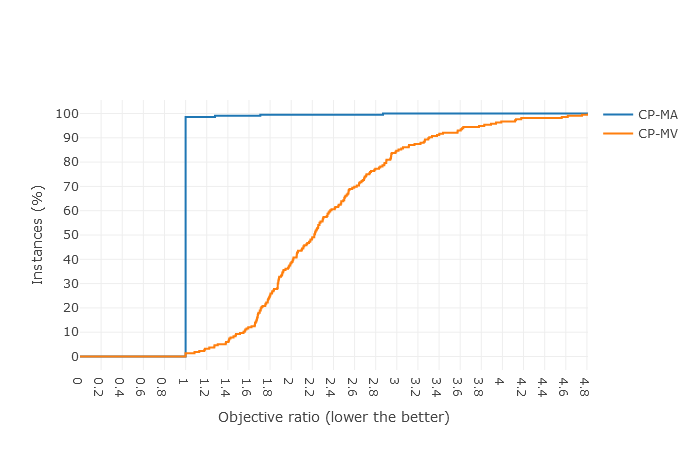
\includegraphics[scale=0.55]{experiments/ma-mv-profile.png}
  \caption{Performance profiles of Most Available and Max Value heuristics [216 instances/30s].}
  \label{experiments:ma-mv-profile}
\end{figure}

We can also see from \autoref{experiments:ma-mv-timeline} that, as the search moves forward, our custom heuristic manages to 
find better solutions faster.

\begin{figure}
  \centering
  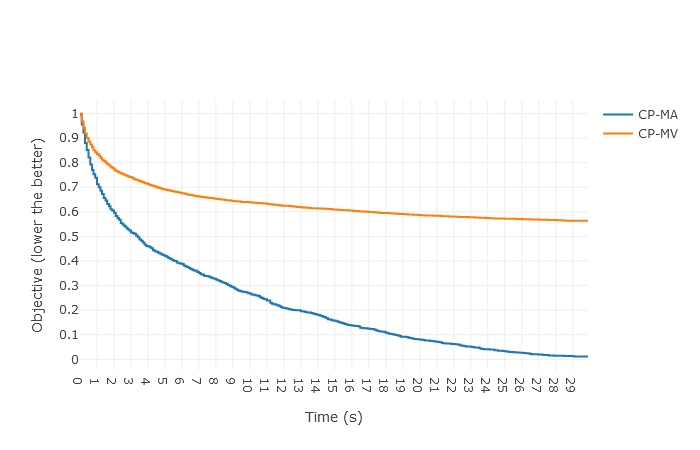
\includegraphics[scale=0.55]{experiments/ma-mv-timeline.png}
  \caption{Timeline of Most Available and Max Value heuristics [216 instances/30s].}
  \label{experiments:ma-mv-timeline}
\end{figure}

Heuristics like the max value are ones of the simpler heuristics to implement but often offers bad performance due to 
the lack of knowledge of the problem.

\paragraph{}

We now compare our static and dynamic most available heuristics together.
\autoref{experiments:ma-ma-d-profile} shows the performance profiles of the dynamic and static most available heuristics.
We can see that the dynamic version of the heuristic outperforms the static one in 90\% of instances after 30s of search.

\begin{figure}
  \centering
  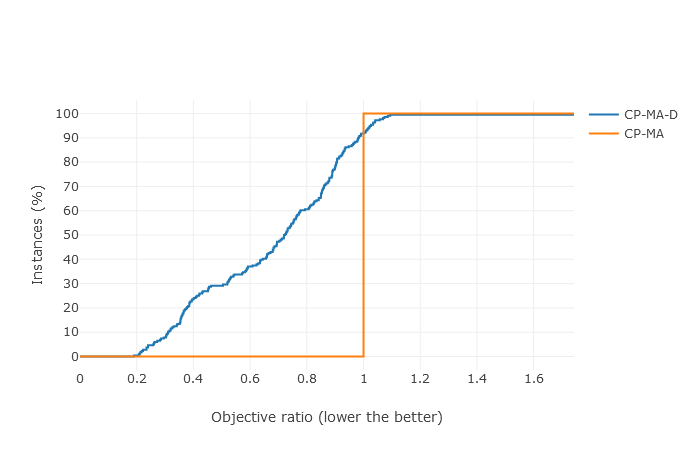
\includegraphics[scale=0.55]{experiments/ma-ma-d-profile.png}
  \caption{Performance profiles of static and dynamic most available heuristics [216 instances/30s].}
  \label{experiments:ma-ma-d-profile}
\end{figure}

Even though the dynamic version needs to process more during the search, we can see from \autoref{experiments:ma-ma-d-timeline} that the time lost 
by this processing is gained back during the search. The first solutions are almost of the same quality but 
as the search moves forward, better solutions are found with the dynamic version. 
This is expected from the implementation of the dynamic version which finds the best worker to assign 
at the current state of the search.

\begin{figure}
  \centering
  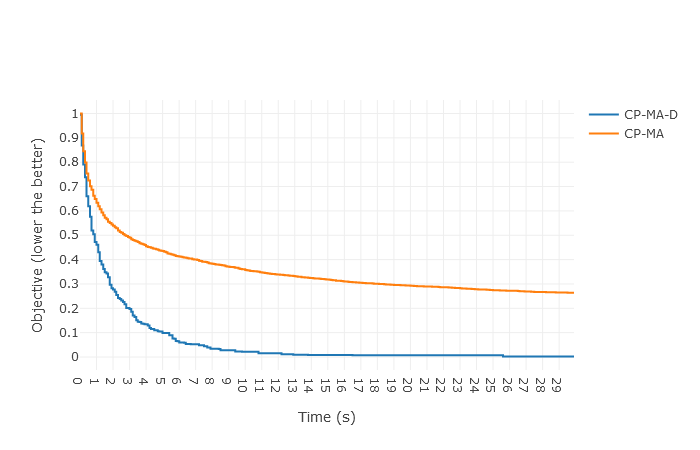
\includegraphics[scale=0.55]{experiments/ma-ma-d-timeline.png}
  \caption{Timeline of static and dynamic most available heuristics [216 instances/30s].}
  \label{experiments:ma-ma-d-timeline}
\end{figure}


\paragraph{}

As our dynamic value heuristic outperforms other tested value heuristics, we assume for the rest of this chapter 
that the value heuristic for the Constraint Programming solver is the dynamic most available.



\subsubsection{Variable heuristic}

In addition to our most available heuristic, we use a variation of the max degree heuristic. 
This heuristic is a first-fail variable heuristic that selects the most constrained unbound variable. However,
as stated in our model in \autoref{section:cpmodel}, skills are not represented with constraints but instead, values 
are removed from the domain at initialization. To express skills as part of the max degree, we simply add the number of 
skills required by a variable to the degree of that variable.


We compare multiple variable heuristics:

\begin{itemize}
  \item Custom Max Degree (MD) heuristic
  \item Min Size (MS) heuristic. The Min Size heuristic simply selects the variable with minimum domain size.
  \item Conflict Ordering Search (COS) heuristic \cite{Gay:COS}
\end{itemize}


Conflict Ordering Search is a variable ordering heuristic that 
reorders variables based on the number of conflicts that happen during the search.
It is a variant to the Last Conflict heuristic which selects the variable which caused the last conflict first.
COS was shown to be the most performant on scheduling problems. 
We will now see how it performs in our problem in comparison with the aforementioned heuristics.

\autoref{experiments:v-heuristics-profile} shows the performance profiles of the objective after 30s for each solver.
We can see that the conflict ordering search and min size heuristics are underperforming in comparison to the max degree heuristic.


\begin{figure}
  \centering
  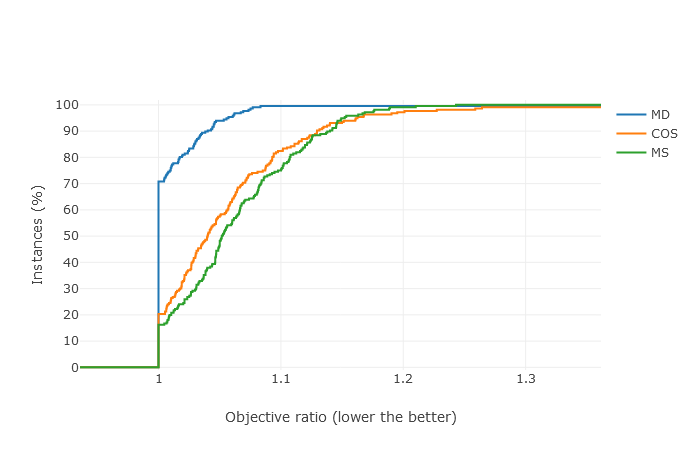
\includegraphics[scale=0.55]{experiments/v-heuristics-profile.png}
  \caption{Performance profiles of COS, Max Degree and Min Size heuristics [216 instances/30s].}
  \label{experiments:v-heuristics-profile}
\end{figure}

However, as we can see from the first five seconds of search in \autoref{experiments:v-heuristics-timeline}, the 
max degree heuristics performs slightly worse than COS and MS for the first second of search. If a solver only runs for 
one second, using COS or MS would be preferable.

\begin{figure}
  \centering
  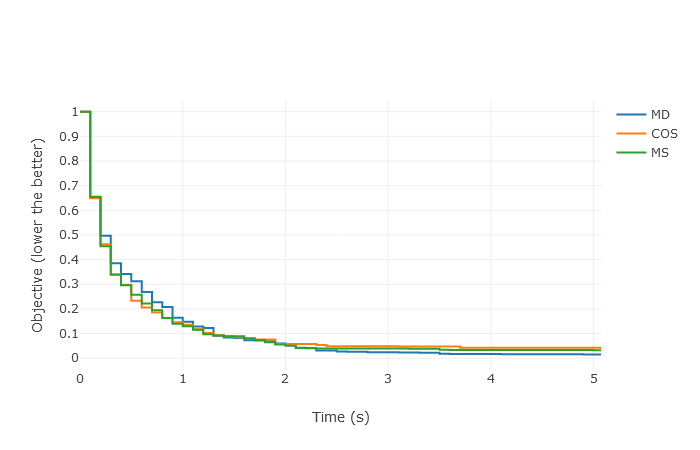
\includegraphics[scale=0.55]{experiments/v-heuristics-timeline.png}
  \caption{Timeline of COS, Max Degree and Min Size heuristics for the first five seconds of search [216 instances/5s].}
  \label{experiments:v-heuristics-timeline}
\end{figure}

\subsection{Comparison between searches}

\subsubsection{Large neighborhood search}


As stated in \autoref{chapter:sota} and \autoref{section:cpmodel}, LNS is used to expand the exploration
of the search tree. We now compare our solver with the use of LNS and without. We also compare multiple 
relaxation methods.


\autoref{experiments:lns} shows the performance profiles of the final objective after 30s of search 
between a standard search and LNS. As expected, we can see that LNS outperforms the standard search 
in every instance. 
\autoref{experiments:lns-oot} shows that the standard search quickly gets stuck
while the LNS manages to find better solutions quickly after relaxing the initial solution.

\begin{figure}
  \centering
  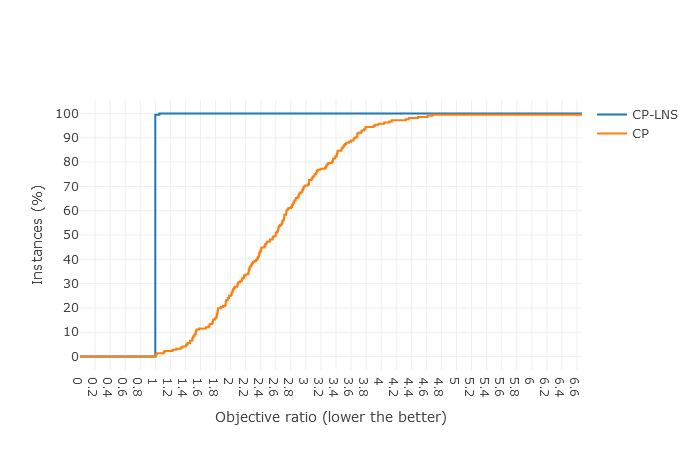
\includegraphics[scale=0.55]{experiments/lns-profile.png}
  \caption{Performance profiles of CP with and without Large Neighborhood Search [216 instances/30s].}
  \label{experiments:lns}
\end{figure}


\begin{figure}
  \centering
  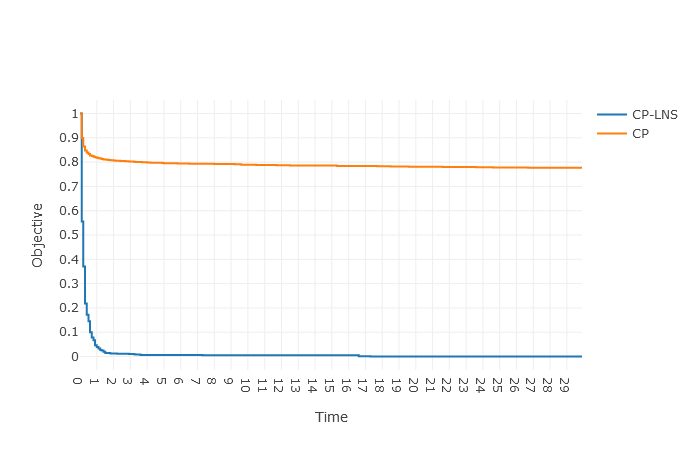
\includegraphics[scale=0.55]{experiments/lns-oot.png}
  \caption{Timeline of CP with and without Large Neighborhood Search [216 instances/3s].}
  \label{experiments:lns-oot}
\end{figure}


The trouble of the standard search to find good solutions is also due to the lack of VO-LNS (\autoref{cp:volns}) as 
this method is an extension of the LNS framework. The standard search can only minimize the weighted sum of sub-objectives
which causes issues when trying to minimize more important (more weighted) sub-objectives first.


\subsubsection{Relaxations}

We also experiment with multiple relaxations in the LNS framework. We compare:

\begin{itemize}
  \item Random relaxation 
    \begin{itemize}
      \item 10\% through 90\% relaxation (CP-Random-N\%)
    \end{itemize}
  \item Propagation based relaxation (CP-Prop)
\end{itemize}

\autoref{experiments:random-relax-profile} first shows performance profiles of all random relaxations 
from 10\% through 90\% relaxation. We observe a trend on this graph that the more relaxation we have,
the worst the objective is. The 10\% and 20\% relaxations offer the best performances after 30s out of all 
the parameters. However, as we can see from \autoref{experiments:random-relax-oot}, the 40\% relaxation 
offers a slightly better objective at the start and the 10\% and 20\% catch up after 9 seconds of search.



\begin{figure}
  \centering
  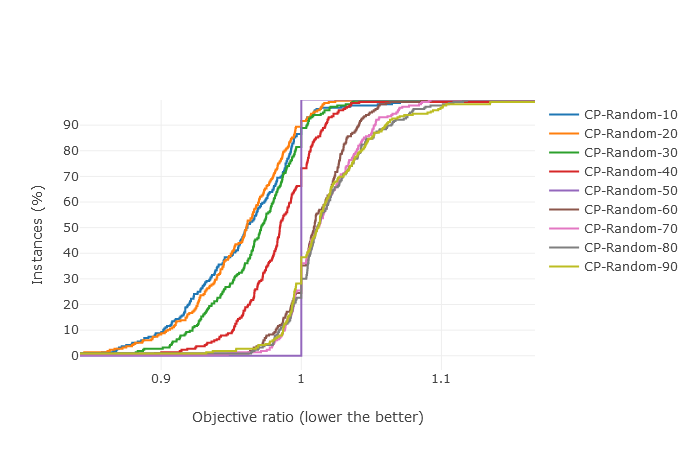
\includegraphics[scale=0.55]{experiments/random-relax-profile.png}
  \caption{Performance profiles of multiple random relaxations [216 instances/30s].}
  \label{experiments:random-relax-profile}
\end{figure}

\begin{figure}
  \centering
  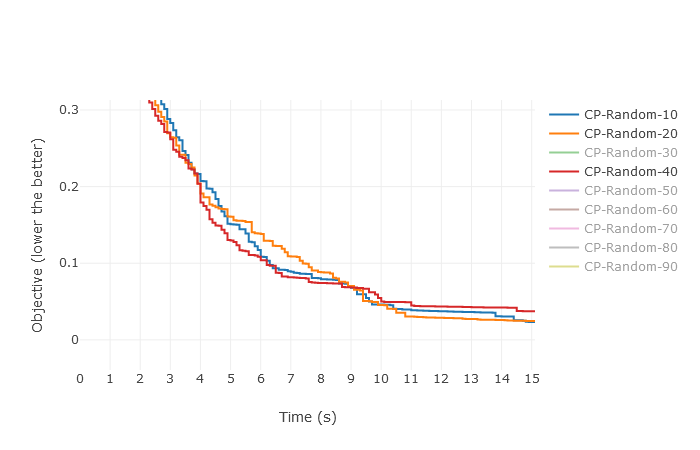
\includegraphics[scale=0.55]{experiments/random-relax-oot.png}
  \caption{Timeline of multiple random relaxations [216 instances/15s].}
  \label{experiments:random-relax-oot}
\end{figure}


We now compare our best random relaxation with a propagation based relaxation.
We choose CP-Random-20 to compare our propagation based relaxation with, as the performances of 
the two best random relaxations are almost the same.
Propagation Guided relaxation takes a neighborhood size parameter, we compare five values for this parameter:

\begin{itemize}
  \item CP-Prop-1/3: the size of the neighborhood to attain is one third of the size of variables.
  \item CP-Prop-1/2: the size of the neighborhood to attain is half the size of variables.
  \item CP-Prop-1: the size of the neighborhood to attain is the size of variables.
  \item CP-Prop-2: the size of the neighborhood to attain is twice the size of variables.
  \item CP-Prop-3: the size of the neighborhood to attain is thrice the size of variables.
\end{itemize}

\autoref{experiments:random-prop-profile} shows the three propagation based relaxations in comparison to CP-Random-20 as baseline.
We can see that all parameters of the propagation based relaxations almost all have the same performances and 
are overall worse than the best random relaxation. Approximately only 5\% of instances are best solved by a propagation based 
relaxation. This makes the random relaxation with 20\% relaxed variables the best out of all tested relaxations.

\begin{figure}
  \centering
  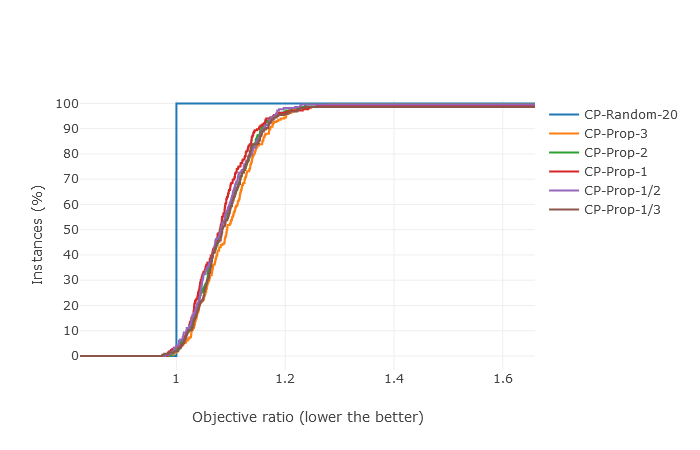
\includegraphics[scale=0.55]{experiments/rand-prop-profile.png}
  \caption{Performance profiles of multiple propagation based relaxations in comparison with the best random relaxation [216 instances/30s].}
  \label{experiments:random-prop-profile}
\end{figure}


\section{Comparison between solvers}

We now start by comparing different solvers together. We experiment with three solvers: 

\begin{itemize}
  \item The Constraint Programming (CP) solver.
  \item The Mixed Integer Programming (MIP) solver.
  \item A combination of CP and MIP (CP+MIP) solvers. We take an initial solution from the CP solver 
  and give it to the MIP solver as start solution. 
\end{itemize}



\autoref{experiments:solvers:profile} 
shows performance profiles with the CP solver as baseline. We can clearly see that 
the MIP solver underperforms for most instances. However, it outperforms the CP solver for approximately
20\% of instances. 

\begin{figure}
  \centering
  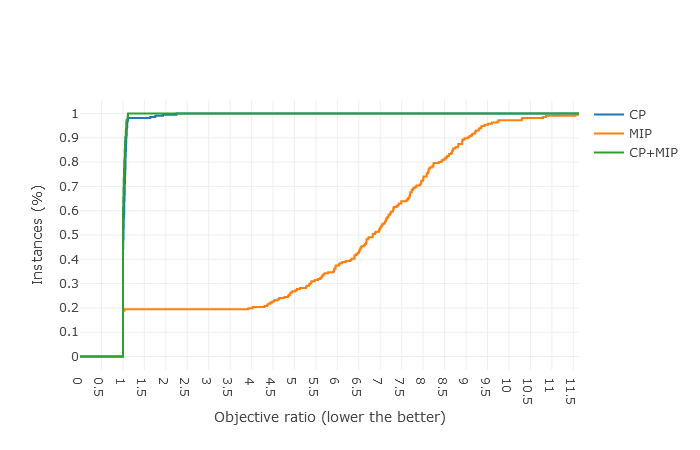
\includegraphics[scale=0.55]{experiments/solvers-profile.png}
  \caption{Performance profiles of CP, MIP and CP+MIP solvers [216 instances/30s].}
  \label{experiments:solvers:profile}
\end{figure}

From \autoref{instances:mip}, we can observe that only small instances are best solved by the MIP solver. 
This highlights the fact that MIP has trouble finding good objectives as the problem size grows.
The problem size directly correlates with the number of binary variables of the MIP model. As an example,
if the problem contains 50 demands over 15 periods with 300 workers and we have 3 workers per demand on average,
we obtain 675.000 binary variables which is more than ten times the number of variables for small instances shown 
in \autoref{instances:mip}. MIP is NP-complete and this high number of variables makes it hard for the solver to find good solutions.


\begin{table}[H]
  \caption{Instance sizes best solved by the MIP solver over the 216 tested instances.}
  \label{instances:mip}
  \centering
  \begin{tabular}[t]{|c|c|c |c|}
    \hline
    \multicolumn{3}{|c|}{Size} & \multicolumn{1}{|c|}{Prop.} \\
    \hline 
    $T$ & $D$ & $W$ & $n$  \\
    \hline 
    \multirow{7}{*}{5} & \multirow{3}{*}{30} & 150 & 8  \\ 
    \cline{3-4}
     &  & 225 & 4  \\ 
     \cline{3-4}
     &  & 300 & 1  \\ 
     \cline{2-4}
     & \multirow{2}{*}{40} & 150 & 8  \\ 
     \cline{3-4}
     &  & 225 & 4  \\ 
     \cline{3-4}
    %  &  & 300 & 8 \\ 
     \cline{2-4}
     & \multirow{2}{*}{50} & 150 & 8  \\ 
     \cline{3-4}
     &  & 225 & 7  \\ 
     \hline
     \multicolumn{3}{|r|}{Total} & 40 \\
      \hline
  \end{tabular}
\end{table}

We can also observe from these performance profiles, and in \autoref{experiments:solvers:profile2}, that 
the CP+MIP solver gives the best objective in 60\% of instances. For the remaining instances, the objective is only worse by a maximum of 10\%. 
The MIP solver performs a lot better when given an initial solution to work with.


\begin{figure}
  \centering
  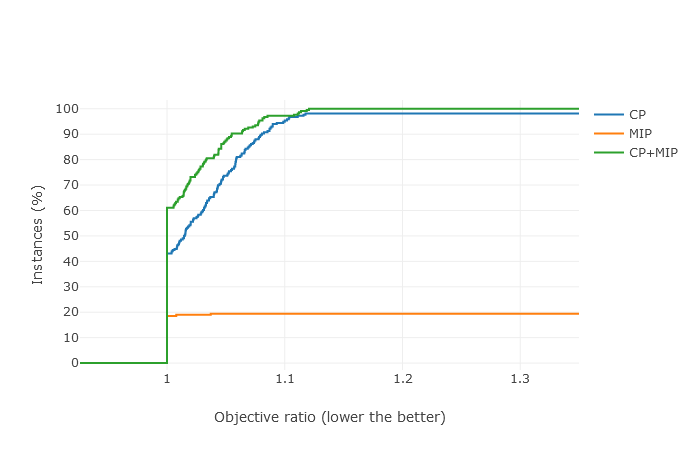
\includegraphics[scale=0.55]{experiments/solvers-profile-zoom.png}
  \caption{Performance profiles of CP and CP+MIP solvers [216 instances/30s].}
  \label{experiments:solvers:profile2}
\end{figure}



\autoref{experiments:solvers:oot} gives the objective per time for the three solvers. As expected from our previous results, the MIP solver does not 
give a good solution after the elapsed time. However, while the CP+MIP solver is slightly better in terms of the final objective, it takes on average 10 seconds 
to reach such objective while the CP solver only takes 1 second to reach an objective really close to the final one.

% Those 20\% match with the small instances proportions in \autoref{instances:proportions}


\begin{figure}
  \label{experiments:solvers:oot}
  \caption{Timeline of CP, MIP and CP+MIP solvers [216 instances/30s].}
  \centering
  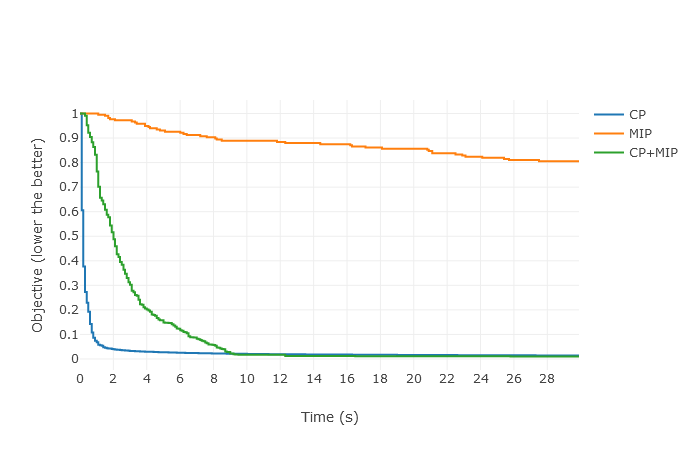
\includegraphics[scale=0.55]{experiments/solvers-oot.png}
\end{figure}


% \begin{figure}
%   \centering
%   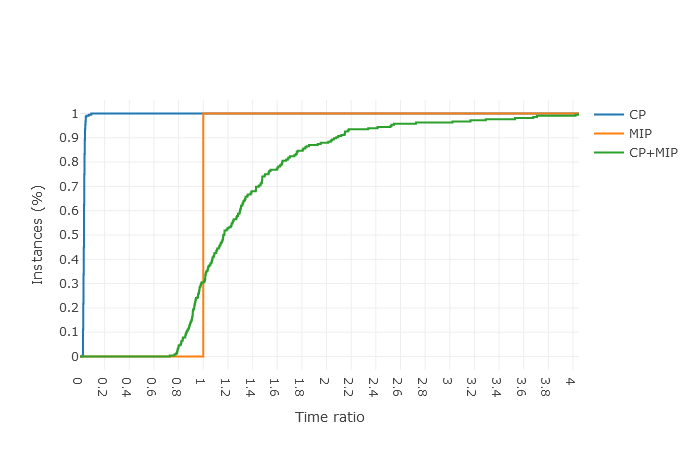
\includegraphics[scale=0.55]{experiments/time-first-sol.png}
%   \caption{Performance profiles of the time on first solution of CP, MIP and CP+MIP solvers [216 instances/First solution].}
%   \label{experiments:first-sol-time}
% \end{figure}


% \begin{figure}
%   \centering
%   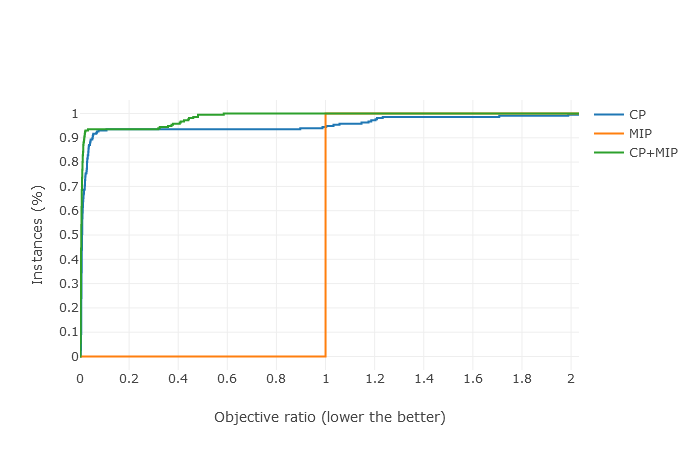
\includegraphics[scale=0.55]{experiments/obj-first-sol.png}
%   \caption{Performance profiles of the objective on first solution of CP, MIP and CP+MIP solvers [216 instances/First solution].}
%   \label{experiments:first-sol-obj}
% \end{figure}




\end{document}

